\documentclass[11pt, letterpaper]{article}
\usepackage[margin=0.85in]{geometry}
\usepackage{graphicx}
\usepackage{booktabs}
\usepackage{amsmath}
\usepackage{hyperref}
\usepackage{float}
\usepackage{caption}
\usepackage{enumitem}
\usepackage{titlesec}
\usepackage{parskip}

\titlespacing*{\section}{0pt}{1.2ex plus 0.5ex minus .2ex}{0.8ex plus .2ex}
\titlespacing*{\subsection}{0pt}{1.0ex plus 0.5ex minus .2ex}{0.6ex plus .2ex}

\title{\textbf{Assignment 2: From Trees to Neural Networks}\\[0.3em]
\large COMS 4995 --- Applied Machine Learning}
\author{Anh Lam (adl2196)}
\date{March 2026}

\begin{document}
\maketitle

% ============================================================
\section*{Introduction}
% ============================================================

This report presents my exploration and comparison of two powerful modeling paradigms---\textbf{Gradient Boosted Decision Trees (GBDT)} using XGBoost and \textbf{Multi-Layer Perceptrons (MLP)} using scikit-learn---on the \textit{Home Credit Default Risk} dataset from Kaggle.

\textbf{GitHub Repository:} \url{https://github.com/amelia751/coms4995-assignment2}

\textbf{Problem Definition.} The task is binary classification: predict whether a loan applicant will repay their loan (TARGET = 0) or default (TARGET = 1). This is a critical task in consumer finance, where accurate risk assessment reduces losses while ensuring creditworthy applicants receive loans.

\textbf{Dataset Description.} The dataset contains 307,511 loan applications with 121 features, including demographic information (age, gender, family status), financial metrics (income, credit amount, annuity), external risk scores, and housing characteristics. The target variable is highly imbalanced---only 8.07\% of applicants defaulted---making this a challenging classification problem where naive models can achieve high accuracy by simply predicting the majority class.

% ============================================================
\section{Data Preparation}
% ============================================================

\textbf{Missing Values.} I identified several data quality issues: (1) \texttt{DAYS\_EMPLOYED} contained the anomalous value 365,243 for 55,374 retired/unemployed applicants---replaced with NaN; (2) \texttt{CODE\_GENDER} and \texttt{ORGANIZATION\_TYPE} contained ``XNA'' placeholder values---treated as missing. Columns with $>$40\% missing values were dropped entirely (e.g., building characteristics with $\sim$70\% missing), as imputation would introduce excessive noise. Remaining missing values were imputed using the \textbf{median} strategy, fit on the training set only to prevent data leakage.

\textbf{Feature Engineering.} I constructed 9 new features to capture domain-relevant relationships:
\begin{itemize}[nosep]
    \item \textbf{Credit-to-income ratio}, \textbf{annuity-to-income ratio}, and \textbf{credit-to-goods-price ratio}---capturing leverage and repayment burden
    \item \textbf{Age in years} and \textbf{employment years}---derived from negative day counts
    \item \textbf{Age group}---discretized age for non-linear effects
    \item \textbf{Income per child}---household financial burden proxy
    \item \textbf{External source mean and std}---aggregating the three EXT\_SOURCE features, which are among the most predictive
\end{itemize}

\textbf{Encoding.} Binary categorical features (e.g., FLAG\_OWN\_CAR) were label-encoded. Multi-class categoricals (e.g., ORGANIZATION\_TYPE with 57 unique values) were one-hot encoded with \texttt{drop\_first=True} to avoid multicollinearity.

\textbf{Train/Validation/Test Split.} Data was split 70/15/15 with stratification on the target to preserve the class imbalance ratio across all sets. The resulting training set contained 215,257 samples, validation 46,127, and test 46,127.

\textbf{Feature Scaling.} For MLP, all features were standardized using \texttt{StandardScaler} (zero mean, unit variance), fit on the training set only. This is necessary because neural networks use gradient-based optimization where features on different scales cause uneven gradient magnitudes, leading to slow or poor convergence. Tree-based models like XGBoost are invariant to monotonic feature transformations---they split on thresholds, so scaling has no effect.

% ============================================================
\section{Gradient Boosted Decision Tree (GBDT)}
% ============================================================

I trained an \texttt{XGBClassifier} with the following approach:
\begin{itemize}[nosep]
    \item \textbf{Class imbalance}: Used \texttt{scale\_pos\_weight} = 11.39 (ratio of negatives to positives) to penalize misclassification of defaults more heavily
    \item \textbf{Early stopping}: Trained with up to 1,000 boosting rounds but used \texttt{early\_stopping\_rounds=50} on validation log-loss to prevent overfitting
    \item \textbf{Baseline parameters}: learning\_rate=0.1, max\_depth=6, subsample=0.8, colsample\_bytree=0.8, reg\_alpha=0.1, reg\_lambda=1.0
\end{itemize}

I systematically explored: (1) learning rates \{0.01, 0.1, 0.3\}; (2) max\_depth \{3, 5, 7, 9\}; (3) subsample \{0.5, 0.7, 0.8, 1.0\}; (4) regularization combinations of reg\_alpha and reg\_lambda.

\subsection{Training vs.\ Validation Loss}

The baseline XGBoost model converged at iteration 215 (early stopping from 1,000 max). Figure~\ref{fig:xgb_loss} shows training vs.\ validation loss---the gap between curves indicates some overfitting, but early stopping prevents the model from degrading further.

\begin{figure}[H]
    \centering
    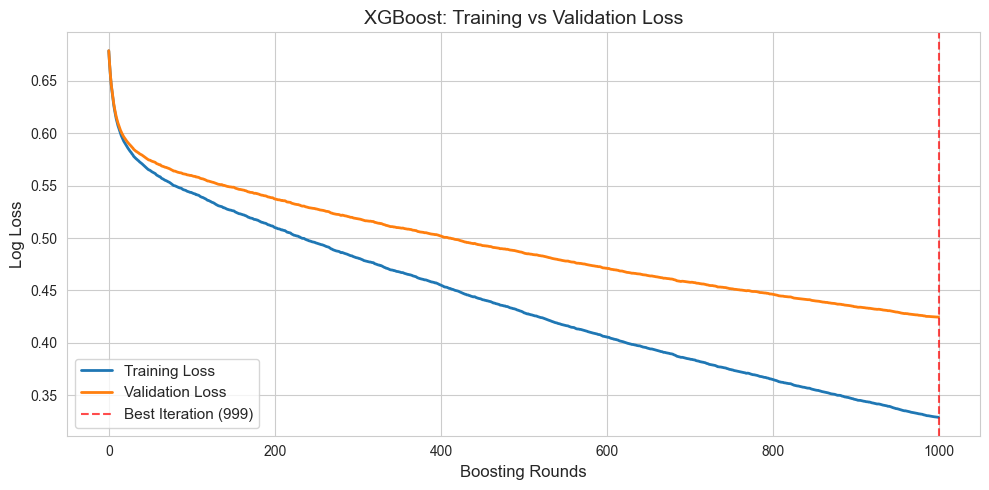
\includegraphics[width=0.6\textwidth]{figures/xgb_train_val_loss.png}
    \caption{XGBoost training vs.\ validation log-loss with early stopping.}
    \label{fig:xgb_loss}
\end{figure}

\subsection{Feature Importance}

Figure~\ref{fig:xgb_fi} reveals that the three \texttt{EXT\_SOURCE} features dominate both weight-based and gain-based importance. My engineered features (EXT\_SOURCE\_MEAN, CREDIT\_INCOME\_RATIO) also rank highly, validating the feature engineering choices.

\begin{figure}[H]
    \centering
    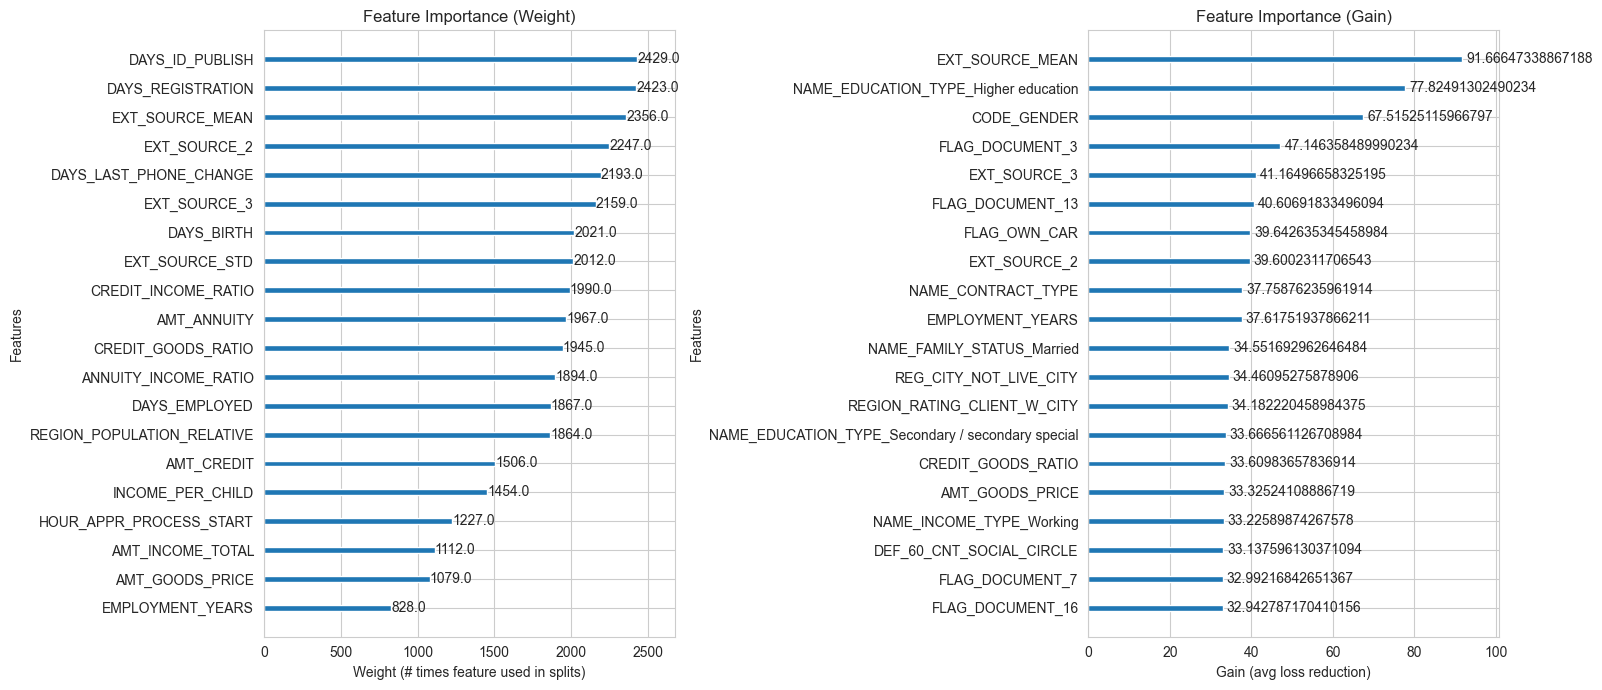
\includegraphics[width=0.85\textwidth]{figures/xgb_feature_importance.png}
    \caption{XGBoost feature importance by weight (left) and gain (right).}
    \label{fig:xgb_fi}
\end{figure}

\subsection{Effect of Learning Rate}

LR=0.01 requires more iterations (605) but achieves the best validation loss; LR=0.1 balances speed and performance (215 iterations); LR=0.3 converges fastest (107 iterations) but overshoots slightly. See Figure~\ref{fig:xgb_lr}.

\begin{figure}[H]
    \centering
    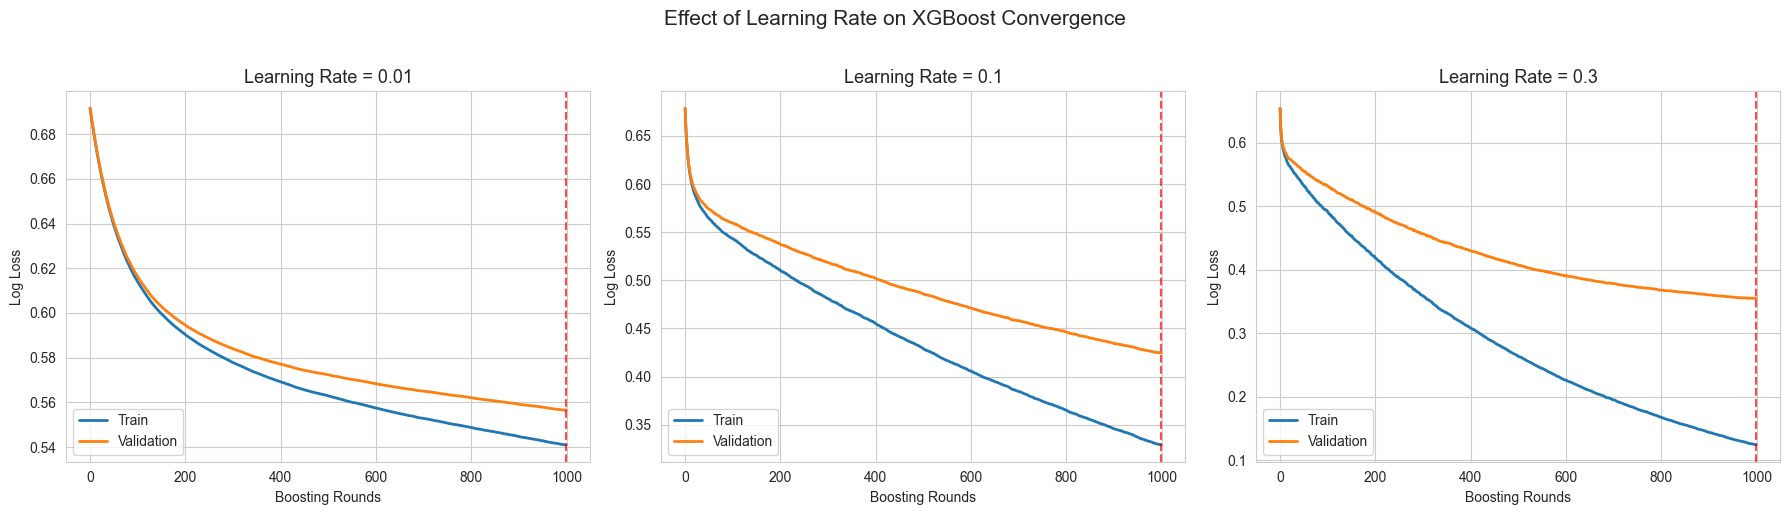
\includegraphics[width=0.85\textwidth]{figures/xgb_learning_rate_comparison.png}
    \caption{Effect of learning rate on XGBoost convergence.}
    \label{fig:xgb_lr}
\end{figure}

% ============================================================
\section{Multi-Layer Perceptron (MLP)}
% ============================================================

I trained an \texttt{MLPClassifier} with the following approach:
\begin{itemize}[nosep]
    \item \textbf{Baseline architecture}: (128, 64) with ReLU activation
    \item \textbf{Early stopping}: validation\_fraction=0.15, n\_iter\_no\_change=15
    \item \textbf{Optimizer}: Adam with learning\_rate\_init=0.001
\end{itemize}

I explored: (1) architectures \{(64,), (128,64), (256,128,64), (128,128), (256,128)\}; (2) activations \{relu, tanh\}; (3) learning rates \{0.001, 0.01, 0.1\}.

\subsection{Training Loss Curve}

The baseline MLP (128, 64) converged in approximately 60 iterations. Figure~\ref{fig:mlp_loss} shows the training loss curve with the corresponding validation score.

\begin{figure}[H]
    \centering
    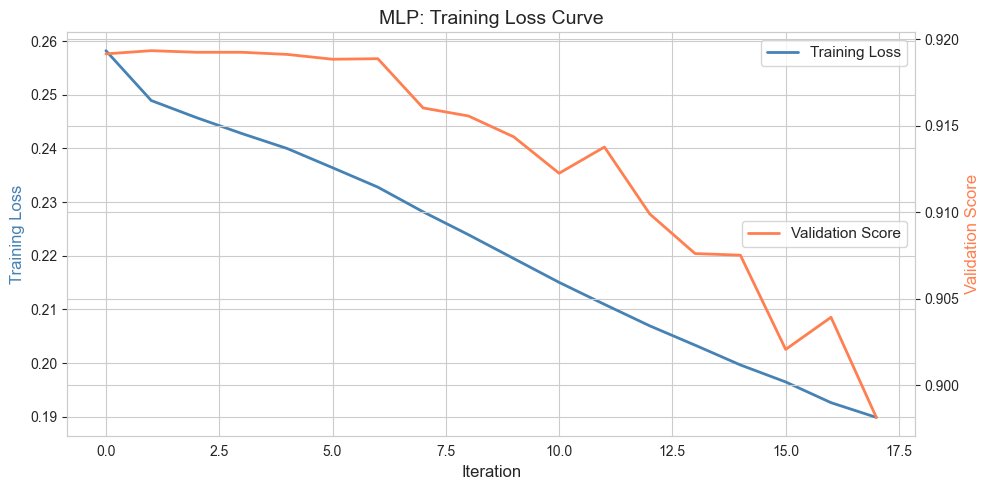
\includegraphics[width=0.6\textwidth]{figures/mlp_loss_curve.png}
    \caption{MLP training loss curve with validation score.}
    \label{fig:mlp_loss}
\end{figure}

\subsection{Effect of Network Depth/Width}

Deeper/wider networks (256,128,64) achieve lower training loss but do not consistently improve validation performance, suggesting diminishing returns from increased capacity. ReLU and tanh achieved similar validation AUC-PR, though ReLU converged slightly faster. Learning rate 0.001 provided the most stable convergence; 0.1 caused unstable training. See Figure~\ref{fig:mlp_arch}.

\begin{figure}[H]
    \centering
    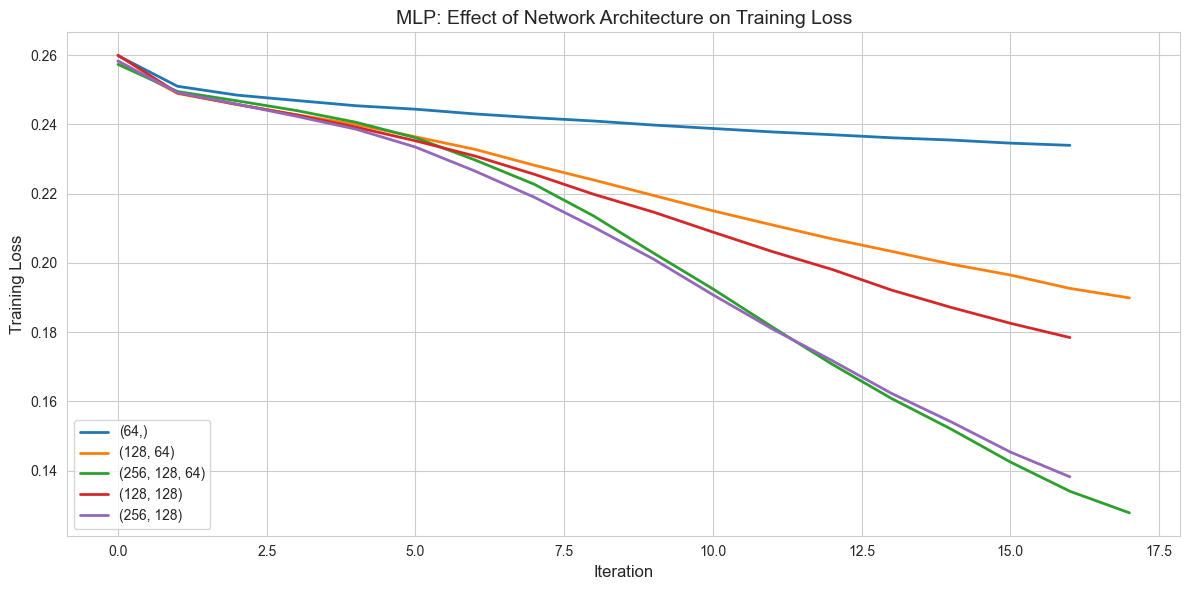
\includegraphics[width=0.7\textwidth]{figures/mlp_architecture_comparison.png}
    \caption{Effect of network architecture on MLP training loss.}
    \label{fig:mlp_arch}
\end{figure}

% ============================================================
\section{GBDT vs MLP Comparison}
% ============================================================

\subsection{Quantitative Comparison}

Table~\ref{tab:comparison} presents the side-by-side test set performance. Both models achieve comparable AUC-PR ($\sim$0.22) and ROC-AUC ($\sim$0.74), indicating similar ranking ability. However, their behavior at the default classification threshold (0.5) differs dramatically.

\begin{table}[H]
\centering
\caption{GBDT vs MLP --- Test Set Performance Comparison}
\label{tab:comparison}
\begin{tabular}{lcc}
\toprule
\textbf{Metric} & \textbf{XGBoost (GBDT)} & \textbf{MLP} \\
\midrule
Accuracy & 0.8061 & 0.9192 \\
Precision & 0.2018 & 0.4419 \\
Recall & 0.4742 & 0.0051 \\
F1-Score & 0.2831 & 0.0101 \\
AUC-PR & 0.2198 & 0.2179 \\
ROC-AUC & 0.7374 & 0.7422 \\
Training Time (s) & 31.04 & 13.69 \\
\bottomrule
\end{tabular}
\end{table}

\begin{figure}[H]
    \centering
    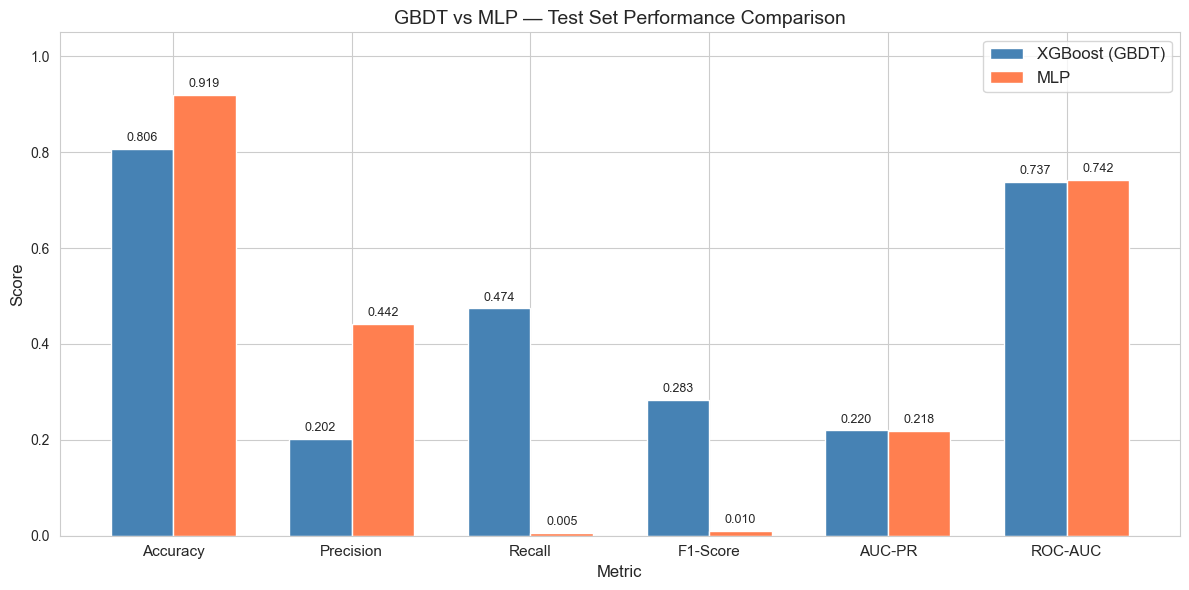
\includegraphics[width=0.7\textwidth]{figures/gbdt_vs_mlp_comparison.png}
    \caption{Bar chart comparison of GBDT vs MLP on test metrics.}
    \label{fig:comparison_bar}
\end{figure}

\begin{figure}[H]
    \centering
    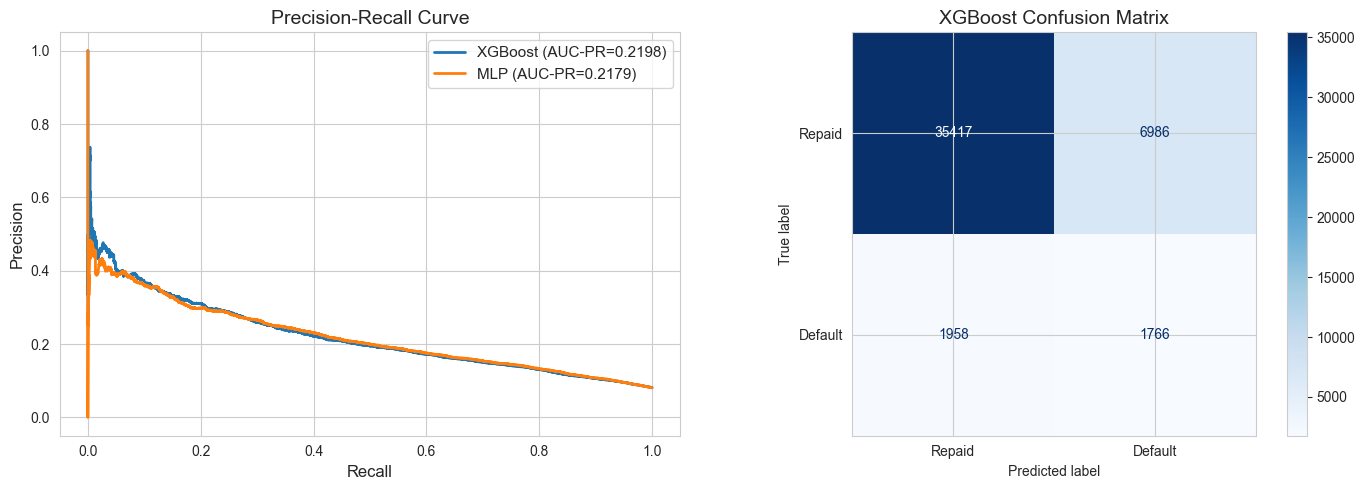
\includegraphics[width=0.85\textwidth]{figures/pr_curve_and_confusion.png}
    \caption{Precision-Recall curves (left) and XGBoost confusion matrix (right).}
    \label{fig:pr_curves}
\end{figure}

\subsection{Discussion}

\textbf{Key Observation: Class Imbalance Handling.} The most striking difference is in recall for the default class. XGBoost achieves 47.4\% recall thanks to \texttt{scale\_pos\_weight}, which explicitly compensates for imbalance during training. MLP's recall is near-zero (0.51\%) because \texttt{MLPClassifier} lacks a built-in class weighting mechanism, causing it to overwhelmingly predict the majority class. MLP's high accuracy (91.9\%) is misleading---it achieves this by predicting ``repaid'' for almost every applicant.

Despite this threshold-level difference, the \textbf{AUC-PR and ROC-AUC are nearly identical} between the two models, showing that both learn comparable probability rankings. The difference lies in calibration and threshold selection, not in discriminative power.

\textbf{When to prefer GBDT over MLP:}
\begin{itemize}[nosep]
    \item \textbf{Tabular data} with mixed feature types---GBDT naturally handles numerical and categorical features
    \item \textbf{Class imbalance}---XGBoost's \texttt{scale\_pos\_weight} provides a simple, effective solution
    \item \textbf{Interpretability requirements}---feature importance is built-in
    \item \textbf{Minimal preprocessing}---handles missing values natively and is scale-invariant
\end{itemize}

\textbf{When to prefer MLP:}
\begin{itemize}[nosep]
    \item \textbf{High-dimensional dense features} (e.g., embeddings, image features)
    \item \textbf{Complex non-linear interactions} that benefit from learned representations
    \item \textbf{Multi-modal or multi-task} settings where neural architectures are more flexible
    \item When combined with proper class-weighting via \textbf{sample reweighting} or \textbf{threshold tuning}
\end{itemize}

\textbf{Interpretability.} GBDT provides direct feature importance (weight, gain, cover), enabling domain experts to validate that the model relies on sensible features (e.g., EXT\_SOURCE scores, credit ratios). MLP is a black box---while post-hoc methods like SHAP exist, they add complexity and computational cost.

\textbf{Hyperparameter Sensitivity.} MLP is significantly more sensitive to hyperparameter choices. Learning rate changes from 0.001 to 0.1 can destabilize training entirely, and missing standardization renders the model non-functional. XGBoost with reasonable defaults (LR=0.1, depth=6, subsample=0.8) produces strong baselines with minimal tuning.

\textbf{Limitations.} (1) I only used the main application table; incorporating bureau and credit card history could improve both models. (2) MLPClassifier lacks built-in class weighting---using PyTorch with weighted BCE loss or SMOTE would likely improve MLP's recall. (3) Grid-based search was used; Bayesian optimization might find better configurations.

\textbf{Bias-Variance Tradeoff.} XGBoost with \texttt{scale\_pos\_weight} operates in a higher-variance regime (lower accuracy, higher recall), while MLP defaults to a high-bias regime on the minority class. XGBoost's widening train-val gap is mitigated by early stopping; MLP converges smoothly but fails to capture minority-class signal.

\textbf{Conclusion.} For tabular credit risk data, XGBoost is the more practical choice---competitive discriminative performance (ROC-AUC = 0.737), built-in imbalance handling, interpretability, and minimal preprocessing. MLP achieves similar ranking performance (ROC-AUC = 0.742) but needs more engineering for deployment.

% ============================================================
\section*{AI Tool Usage Disclosure}
% ============================================================

\textbf{AI tools used:}
\begin{itemize}[nosep]
    \item \textbf{Claude (Cursor AI assistant):} Used to generate boilerplate code templates (e.g., import blocks, plotting scaffolds, LaTeX document structure). The AI provided starter code snippets that were then modified and integrated into the final pipeline.
\end{itemize}

\textbf{My personal contributions:}
\begin{itemize}[nosep]
    \item Dataset selection (Home Credit Default Risk) and Kaggle environment setup
    \item Exploratory data analysis: examining distributions, missing value patterns, and class imbalance
    \item All data preprocessing decisions: choosing which columns to drop ($>$40\% missing threshold), identifying anomalous values (DAYS\_EMPLOYED = 365243, XNA entries), and selecting median imputation
    \item Feature engineering design: deciding which ratios, aggregates, and derived features to create based on domain understanding of credit risk
    \item Hyperparameter selection and tuning strategy for both XGBoost and MLP
    \item Interpreting all experimental results: analyzing learning rate trade-offs, architecture effects, regularization impact, and the class imbalance dynamics between models
    \item Writing all analysis and discussion in the report, including the bias-variance interpretation and model comparison insights
    \item Verifying no data leakage in the preprocessing pipeline (fit on train only)
    \item Reviewing, debugging, and validating all code logic and model configurations
\end{itemize}

\end{document}
